\header{
    \section{Faluchards d'abord} \label{faluchardes-d-abord}
    %
    
    \insertComment{Sur l'air de "Les Copains d'abord" de Georges Brassens (1964).}{}
}

\enluminure{4}{\href{https://www.youtube.com/watch?v=CWJmBBxJlig}{N}}{on} ce n'étaient pas des fachos
\\Des emmerdeurs, ni des idiots
\\Qu'on le dise aux faiseurs de tort
\\Aux faiseurs de tort
\\Ils rigolaient en jeunes fêtards
\\Dans les soirées et dans les bars
\\Et s'app'laient faluchards d'abord
\\Faluchards d'abord
\\\\Et cet amour de la nuit
\\C'est surtout pas d'la connerie
\\N'en déplaise à celui qui dort
\\A celui qui dort
\\Et de loin on préférait boire
\\Quand enfin arrivait le soir
\\Sur l'alcool ils y allaient fort
\\Faluchards d'abord
\\\\C'était pas qu'une simple mode
\\Nous respections tous le code
\\Celui de chez nous et d'ailleurs
\\Chez nous et d'ailleurs
\\Et ces Grands Maîtr' ou Chambellans
\\C'étaient bien tous les garants
\\De ce qu'on appelait alors
\\Faluchards d'abord
\\\\C'était pas les mêmes non plus
\\De tous côtés z'étaient issus
\\Mais ils s'aimaient quel que soit le bord
\\Quel que soit le bord
\\Science, éco, droit, pharmacie
\\C'était vraiment tous des amis
\\Et ils criaient bien haut et fort
\\Faluchards d'abord
\breakpage
C'était une grande famille
\\Des garçons et des jolies filles
\\C'est pas ce qui manquait alors
\\Qui manquait alors
\\Y avait toujours de la tendresse
\\De la joie et de l'ivresse
\\Quand on allait au "Chamois d'Or"
\\Faluchards d'abord
\\\\Au rendez-vous pour les baptêmes
\\L'esprit restait toujours le même
\\Amour et respect d'la faluche
\\Respect d'la faluche
\\Bien sûr jamais au grand jamais
\\Sa flamme chez nous ne s'éteignait
\\Cent ans après coquin de sort
\\Elle brillait encore
\\\\Des bringueurs j'en ai vu beaucoup
\\Mais ceux qui étaient les plus fous
\\Qui étaient toujours les plus forts
\\Toujours les plus forts
\\Rigolaient en jeunes fêtards
\\Dans les soirées et dans les bars
\\Et s'app'laient faluchards d'abord
\\Faluchards d'abord
\begin{center}
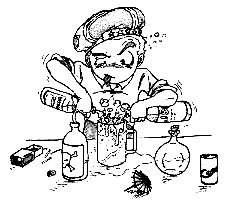
\includegraphics[width=0.6\textwidth]{images/faluchard.png}
\end{center}

\breakpage